\usetikzlibrary{calc}
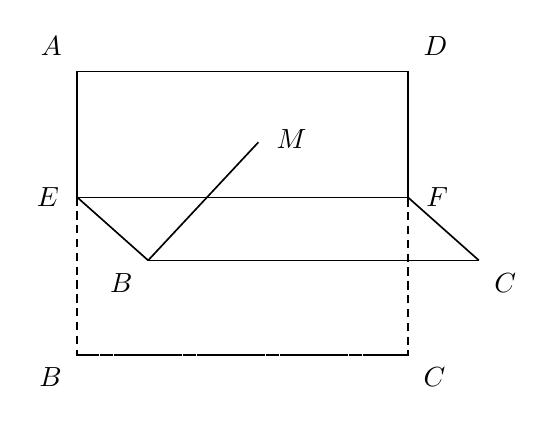
\begin{tikzpicture}[x=1cm,y=1cm,line width=.6pt,font=\normalsize]
% upper rectangle AEFD, lower folded parallelogram + dashed pre-fold
\coordinate (A) at (0,3.2);
\coordinate (D) at (4.2,3.2);
\coordinate (E) at (0,1.6);
\coordinate (F) at (4.2,1.6);
\coordinate (B) at (0.9,0.8);
\coordinate (Cs) at (5.1,0.8);
\coordinate (B0) at (0,-0.4);
\coordinate (C0) at (4.2,-0.4);
\coordinate (M) at (2.3,2.3);
% upper rectangle solid
\draw (A) -- (D) -- (F) -- (E) -- cycle;
\draw (E) -- (F);
% folded solid lower part E-B-Cs-F
\draw (E) -- (B);
\draw (B) -- (Cs);
\draw (F) -- (Cs);
% B-M segment crossing EF
\draw (B) -- (M);
% dashed pre-fold rectangle
\draw[densely dashed] (E) -- (B0) -- (C0) -- (F);
\draw[densely dashed] (B0) -- (C0);
% labels
\node[anchor=south east,xshift=-2pt,yshift=2pt] at (A) {$A$};
\node[anchor=south west,xshift=2pt,yshift=2pt] at (D) {$D$};
\node[anchor=east,xshift=-3pt] at (E) {$E$};
\node[anchor=west,xshift=3pt] at (F) {$F$};
\node[anchor=north east,xshift=-2pt,yshift=-1pt] at (B) {$B$};
\node[anchor=north west,xshift=2pt,yshift=-1pt] at (Cs) {$C$};
\node[anchor=north east,xshift=-2pt,yshift=-1pt] at (B0) {$B$};
\node[anchor=north west,xshift=2pt,yshift=-1pt] at (C0) {$C$};
\node[anchor=west,xshift=3pt,yshift=1pt] at (M) {$M$};
\end{tikzpicture}
